\documentclass{alex_gp}

\name{Alexander Helbok}
\course{Grundpraktikum}
\hwnumber{1}


\begin{document}

\begin{myfigure}{Datenaufzeichnung}{11}
	\begin{wrapfigure}{r}{0.5\textwidth}
			\vspace{-1em}
			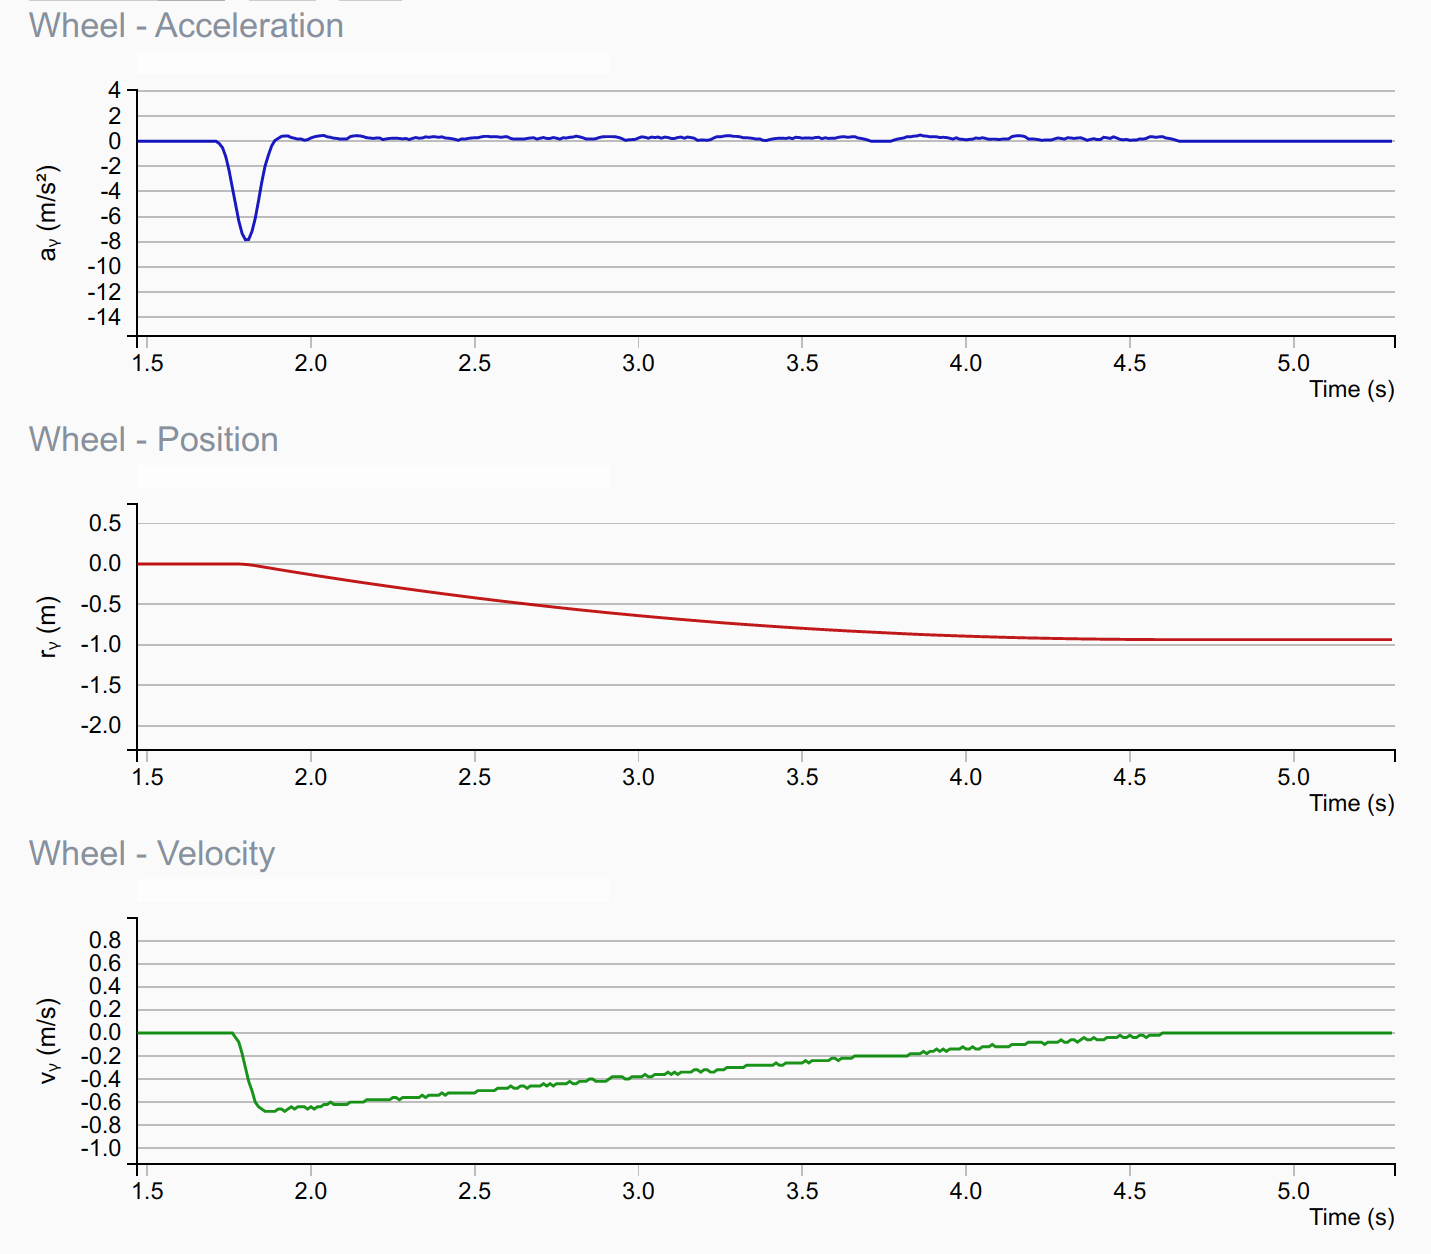
\includegraphics[width=0.5\textwidth]{Versuch1 - 2}
			\caption{Von oben nach unten sind Beschleunigung, Ort und Geschwindigkeit des Messgeräts auf die Zeit aufgetragen. Nur der relevante Zeitabschnitt wird dargestellt.}
	\end{wrapfigure}
	In der nebenstehenden Abbildung sieht man jeweils die Beschleunigung, die Geschwindigkeit und den Ort des IOLab Messgeräts auf die Zeit aufgetragen. 
	Der oberste Plot zeigt die Beschleunigung in Bewegungsrichtung, in Rot sieht man die Position in Bezug auf die Anfangslage, und der grüne Graph stellt die Geschwindigkeit des Geräts dar. \par
	
	\indent Das Gerät befindet sich anfänglich in Ruhe bis der Stoß kommt, was sich im Beschleunigungs- und Geschwindigkeitsgraphen als starker negativer Anstieg erkenntlich macht. 
	Nach dem Stoß geht die Beschleunigung zu etwas über 0 zurück und die Geschwindigkeit des Geräts verringert konstant (aufgrund von Reibung). Der Ortsgraph flacht mit der Zeit ab, da das IOLab Gerät immer langsamer wird und somit weniger Weg in der gleichen Zeit zurücklegt. \par
	
	Zum Schluss steht das Gerät still und die Graphen nehmen eine konstante ein.
\end{myfigure}
\newpage
\begin{mybox}{Analysewerkzeuge}
	\begin{minipage}[0.4\textheight]{\textwidth}
		\begin{multicols}{2}
			\centering
			\begin{tabular}{c| c || c  c  c} 
			\hline
				\multicolumn{2}{c ||}{} & \( \mu \) & \( \sigma \) & s \\ [0.5ex] 
			\hline\hline
				\multirow{3}{*}{\rotatebox{90}{Intervall 1}} & 
				\( \vec{x} \) & -0.479 & 0.036 & -0.47 \\ 
				& \( \vec{v} \) & -0.475 & 0.022 & 0.26 \\
				& \( \vec{a} \) & 0.270 & 0.071 & -0.52 \\ [1ex] 
			\hline
				\multirow{3}{*}{\rotatebox{90}{Intervall 2}} & 
				\( \vec{x} \) & -0.684 & 0.026 & -0.34 \\ 
				& \( \vec{v} \) & -0.347 & 0.020 & 0.23 \\
				& \( \vec{a} \) & 0.250 & 0.090 & -0.44 \\ [1ex] 
			\hline
				\multirow{3}{*}{\rotatebox{90}{Intervall 3}} & 
				\( \vec{x} \) & -0.825 & 0.017 & -0.22 \\ 
				& \( \vec{v} \) & -0.222 & 0.020 & 0.25 \\
				& \( \vec{a} \) & 0.211 & 0.12 & -1.00 \\ [1ex] 
			\hline
			\end{tabular}
		\columnbreak
			\begin{figure}[H]
				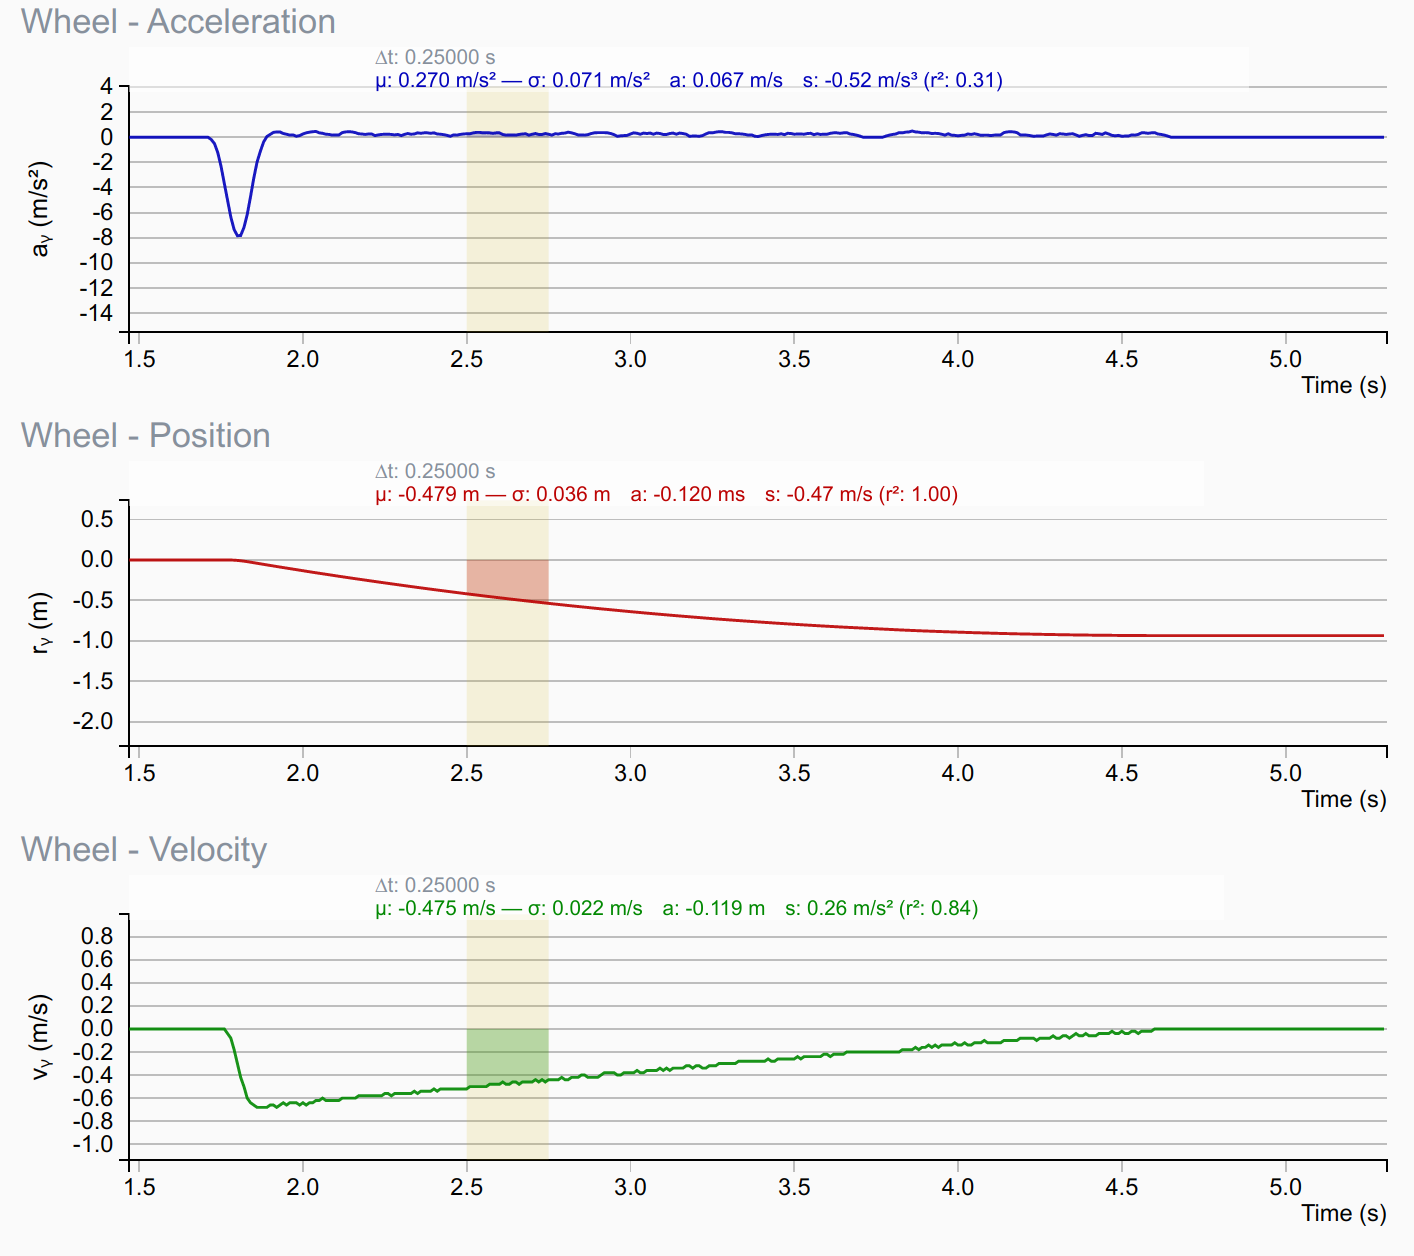
\includegraphics[width=0.5\textwidth]{Versuch1 - 3}
				\caption{Von oben nach unten sind Beschleunigung, Ort und Geschwindigkeit des Messgeräts auf die Zeit aufgetragen. }
			\end{figure}
		\end{multicols}
	\vspace{1em}
	\end{minipage}
%		
		\noindent Es wurden 3 Intervalle ab \( t = 2.5 \unit{s}, 3 \unit{s}, 3.5 \unit{s} \) und Länge \( \Delta t = 0.25 \unit{s} \) gewählt und jeweils der Mittelwert \( \mu \), die Standardabweichung \( \sigma \) und die Steigung \( s \) einer angepassten Gerade berechnet. Diese Gleichungen
		\begin{equation}
			\vec{v} = \dv{\vec{x}}{t};\quad \vec{a} = \dv{\vec{v}}{t}
		\end{equation}
		stellen einen Zusammenhang zwischen Ort, Geschwindigkeit und Beschleunigung her. In unserem Fall können wir \( \vec{x}, \vec{v}, \vec{a} \) direkt messen 
\end{mybox}
\newpage
\begin{mybox}{Analyse}
	\begin{figure}[H]
		\vspace{-0.5cm}		
		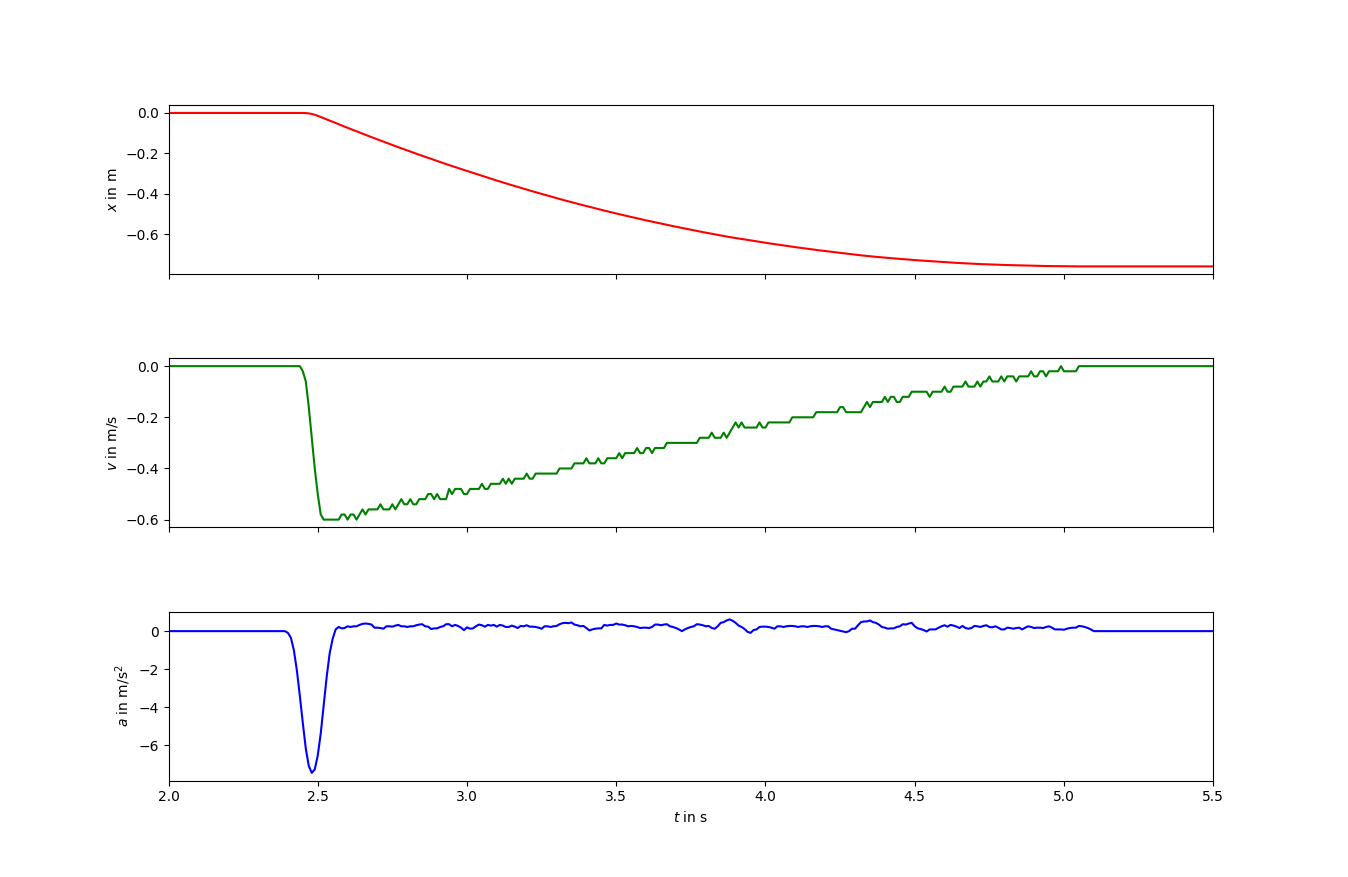
\includegraphics[width=\textwidth]{Versuch1 - 1}
		\caption{Von oben nach unten sind Ort, Geschwindigkeit und Beschleunigung des Messgeräts auf die Zeit aufgetragen. Nur der relevante Zeitabschnitt wird dargestellt.}
	\end{figure}
\end{mybox}

\end{document}